\documentclass[twocolumn]{article}

\usepackage{parskip}
\usepackage{titling}
\usepackage{graphicx}
\usepackage[backend=bibtex,
style=numeric
]{biblatex}
\addbibresource{../bibliography}

% Document metadata
\title{
    GEOG 5551 Term Project: Project Paper
}
\author{
    Aamdal, Haakon\\
    \texttt{aamda001@umn.edu}
}


% Margins
\topmargin=-0.45in
\evensidemargin=0in
\oddsidemargin=0in
\textwidth=6.5in
\textheight=9.0in
\headsep=0.25in

\begin{document}
\maketitle

\section{Introduction}
\label{sec:Introduction}
According to a white paper published by Bell Labs \cite{Bell_Labs2013-st} on internet traffic growth, the end-user internet connection traffic demand is forecasted to increase by 3.7 from 2012 to 2017. Nearly all of the demand is forecasted to come from residental and business fixed internet connections. There's over 30 internet service providers (ISPs) in the United States \cite{noauthor_undated-uf}, resulting in a highly competitive market with low margins of profit. This paper explains how an ISP can take advantage of a geographical information system (GIS) to maximize profit and minimize risk in the process of finding new customer to connect to their existing network.

The system proposed in this paper will be a tool for locating new customers for an ISP, that is customers not connected to the ISP's current infrastructure, with the most potential. A GIS is advantageous for this task, because the ISP would be interested in physical location of businesses and households most likely to sign up for a new high speed fixed internet connection service. In order to find the customers with the most potential, the system will use several attributes of the households and businesses, like the total income/revenue or number of residents/employees. In addition to this, the cost of installing new customers will have to be taken into consideration when ranking profitability and potential. Clustered customers have lower costs per installation. In addition, the closer the customer to existing infrastructure, the better.

\section{Data}
\label{sec:Data}
This project is highly dependent on good data sources to be successful. Data is collected from a number of sources, all listed in this section.

\begin{figure}
  \centering
  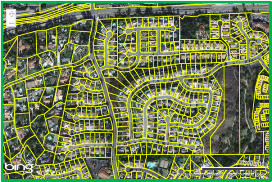
\includegraphics[width=0.45\textwidth]{img/parcel.png}
  \caption{Parcel data from Digital Map Products}
  \label{fig:parcel}

\end{figure}
\paragraph{Parcel data}

\label{par:Parcel data}
A quick google search reveals that there exists several companies that sells parcel data for the United States. Digital Map Products \footnote{http://www.digmap.com/} is one of them. They deliver vector and raster digital parcel boundaries for over 120 million US parcels. The data also contains the assessors parcel number (APN), which makes it possible to link the parcels with tax data. Their vector dataset would be most useful for this application, and can be downloaded in the standard ArcGIS Shapefile format. The dataset is however not free, you need to contact them to get an offer. An example map is shown in Figure~\ref{fig:parcel}.

\begin{figure}
  \centering
  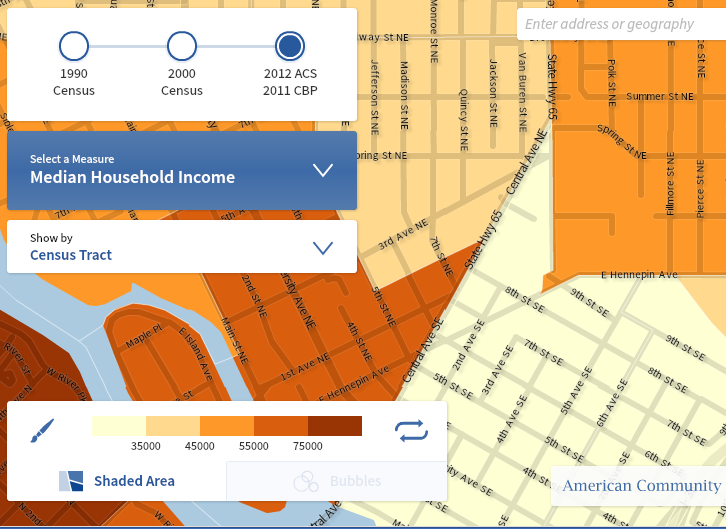
\includegraphics[width=0.45\textwidth]{img/census.png}
  \caption{Median household income from the United States Census Bureau for Minneapolis NE. The data is divided by census tracts.}
  \label{fig:census}
\end{figure}
\paragraph{US Census data}
\label{par:Us Census data}
The United States Census Bureau can provide data on several households attributes, including average income, average number of children and precentage of population with high school diploma. Since the US Census only samples a fraction of the total population, and are required to conserve anonymity, their data are divided into census tracts/blocks or even counties. Please see Figure~\ref{fig:census} for an example of how the census tracts are divided. All of the data from the US Census are free of charge.

\begin{figure}
  \centering
  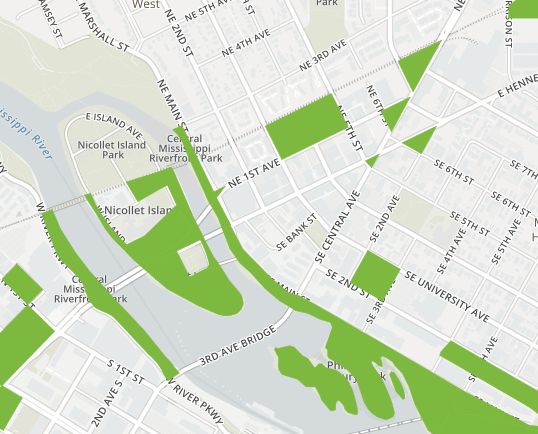
\includegraphics[width=0.45\textwidth]{img/nbm.png}
  \caption{The National Broadband Map showing which areas in Minneapolis NE that only have one or two broadband suppliers.}
  \label{fig:nbm}
\end{figure}
\paragraph{National Broadband Map}
\label{par:National Broadband Map}
The National Broadband Map\footnote{http://www.broadbandmap.gov/} is an updated dataset to where you can search, analyze and map broadband availability across the United states. The data includes broadband speed, broadband technology, number of broadband providers and more. It can map areas where there are fewer broadband suppliers than others. It also contains data which correlates bandwidth speed with demographics, like population density, age, income or education. The National Broadband Map is free of charge.

\begin{figure}
  \centering
  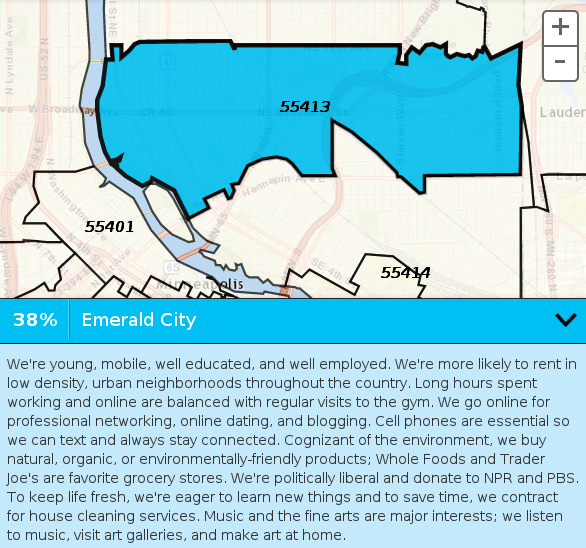
\includegraphics[width=0.45\textwidth]{img/tapestry.png}
  \caption{The Esri Tapestry data for ZIP 55414. The data explains the average citizen of the area, including leisure time activities, political standpoints and buying patterns.}
  \label{fig:tapestry}
\end{figure}
\paragraph{Esri Tapestry Segmentation}
\label{par:Esri Tapestry Segmentation}
Esri provides a dataset named Esri Tapestry Segmentation\footnote{http://www.esri.com/landing-pages/tapestry/} aiming to improve understading of people's lifestyle choices, what they buy and how they spend their free time. The tapestry classifes U.S. residential neighborhoods into 67 unique segments based on socioeconomic and demographic characteristics. Each segment offers a picture of the average citizen, revealing information on leisure activities and buying patterns. See Figure~\ref{fig:tapestry}. The tapestry data is available for purchase from Esri.

\paragraph{Business data}
\label{par:Business data}
The United States Census Bureau also provides data about businesses\footnote{http://www.census.gov/econ/susb/}, which includes number of establishments, employment and annual payroll for most U.S. businesses. This data is very coarse grained, as it is divided into census tracts or counties. A better option would be the US Business Locations and Business Summary database\footnote{http://www.esri.com/data/esri\_data/business-overview/business} from Esri. This database gives you the location of all businesses in the United States, as well as relevant attributes like annual sales and number of employees. The business data is available for purchase from Esri and can be downloaded in vector format as points.

\begin{figure}
  \centering
  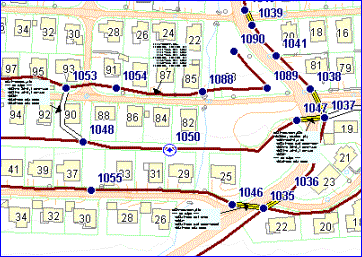
\includegraphics[width=0.45\textwidth]{img/telme.png}
  \caption{Sample documentation from the TelMe software. Different network infrastructure like cables, connections and hubs are documented spatially.}
  \label{fig:telme}
\end{figure}
\paragraph{Existing network infrastructure}
\label{par:Existing network infrastructure}
Another important part of the system is the documentation of the ISP's existing network infrastructure. At a minimum, the application requires all relevant components, like hubs, connectors and cables, to be documented spatially. This data should be in vector format. There exists several products out there to help documenting cable infrastructure. The TelMe\footnote{https://micado.no/index.php?cont=cont/3TelMe\_TM.html} software from Micado AS is one of them, and an example of spatial documentation is shown in Figure~\ref{fig:telme}.


\subsection{Preparing the data for analysis}
\label{sub:GIS operations for combining data}
\begin{figure}
  \centering
  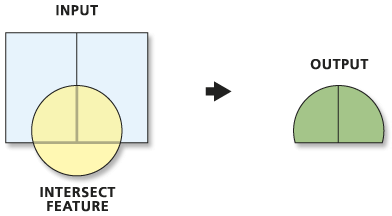
\includegraphics[width=0.45\textwidth]{img/intersect.png}
  \caption{Splitting spatial features and combining attributes. Courtesy of \cite{noauthor_undated-dw}.}
  \label{fig:intersect}
\end{figure}
Since the data comes from so many different sources, it needs to be combined before it can be used in further analysis. We would like to combine the household and business data with the other more coarse-grained data, like data from the National Broadband Map and Census data. An easy way of doing this would be to do use the overlay technique Intersect. The result of this would be the coarser grained data split into smaller pieces and combined with the businesses or parcels, effectively expanding the source tables with new attributes. Please see Figure~\ref{fig:intersect} for how the intersect operation works.

It is however very important to be aware of the pitfalls by combining coarse grained information with fine grained. For example, all households would be assigned an average income. However, this income does not reflect the average income of the house, it is still the average income of the census tract the household belongs to. This needs to be taken into consideration when analysing the data. However, if the data sources are split up differently, you will get a tighter classification of each parcel. For instance, you can have two households with the same income (because they are in the same census tract), but have different number of broadband suppliers, because the National Broadband Map splits up its blocks differently that the US Census.


Additionally, the ISPs network infrastructure might not be documented spatially. Depending on the format of the current documentation, getting the required vector data might include:
\begin{itemize}
  \item If the network is documented on paper maps with drawing and sketches, these maps would need to be scanned and georeferenced. Since we need vector data, manual digitizing of relevant map features like boxes, cables and connectors might need to be digitized/extracted manually.
  \item If the network is documented non-spatially, like in a spreadsheet, all relevant points would have to be geocoded. The documentation might already include coordinates. This would require us to convert the aspatial table to a spatial one using the x and y attributes. If the documentation does not have coordinates, but rather addresses, these could be looked up and be put in the map. If documentation about cable endpoint exsists, these could be drawn as lines between the corresponding geocoded points.
  \end{itemize}

Lastly, due to cluster analysis explained in Section \ref{sec:Methods}, we would like all of our household and businesses to be points rather than polygons. This transformation would simply replace the polygon of each feature with the centroid point, keeping all the attributes intact.


\section{Potential and profitability}
\label{sec:Potential and profitability}
Even with a wide range of data available, it's not obvious how to use them. This section aims to explain which attributes are relevant for ranking new customers in terms of potential and profitability.

\subsection{Household potential}
\label{sub:Potential}

\paragraph{Analyzing data from the Broadband Network Map}
\label{sub:Analyzing data from the Broadband Network Map}
The National Broadband Map provides a map showing the correlation between broadband speed and demographics data, more specifically for population density, age, income and education. By visually inspecting the map with the different categories, one can come up with the following conclusions:
\begin{itemize}
  \item Median age does not correlate with the broadband speeds. 
  \item Median income correlates to broadband speeds. The higher the income, the higher speed.
  \item The precentage of people with high school diploma correlates to broadband speed.
\end{itemize}
Even though this visual inspection is not very accurate, it still pinpoints attributes worth looking at when looking for customers that would like to improve it's internet connection.

\paragraph{Internet usage}
\label{sub:Internet usage}
The \textit{PewResearch Internet Project} provides data about U.S. internet usage \cite{noauthor_2013-ev}. Although this statistics does not explicitly state the type of connection (speed, fixed vs. mobile), it's still a valid guideline for pointing out users with high potential. The report backs up the observation from Section \ref{sub:Analyzing data from the Broadband Network Map}: The more eductated and well paid population got more potential. In addition to this, the statistic also shows that the younger the population, the higher internet usage.

\paragraph{The Esri Tapestry Segmentation}
\label{sub:The Esri Tapestry Segmentation}
One could also use the Esri Tapestry Segmentation directly. This data provides a definition of each customer segment. All segment descriptions could be analysed with broadband connection demand in mind. For instance, the ISP could look for customer segments describing people with a high use of internet traffic intensive applications like gaming and streaming.

\subsection{Business potential}
\label{sub:Businesses}
The research for project have not been able to find any sources on business potential when it comes to demand for high speed internet connections. One could still normal intuition to do a profitiability assessment. The more employees, the higher demand. In addition, high yearly revenue will also be an indicator of purchasing power.

\subsection{Profitability}
\label{sub:Profitability}
The cost of installing the new customers will also have to be taken into consideration when ranking profitability and potential. According to a paper on economics of fibre to the home by Weldon, M. K. and Zane, F. \cite{Weldon2003-xq}, the population density of the area will affect the total cost. More specifically, the lower population density, the higher the cost of the new network infrastructure. In other words, potential customers clustered together with other potential customers is will be cheaper to install. Additionally, the paper states that labor costs for digging down the cables in a trench (trenching) is a big part of the expenses, so proximity to already existing network infrastructure should be considered when finding new customers. 

Another aspect of customer profitability is the precence of other broadband providers in the area. If the households or businesses are ranked as very potential customers, it's likely some other ISPs already supply broadband connections to them. Expanding the network in that area would be associated with high risk, as it is not very likely that the customers would like to change a broadband supplier they're already satisfied with, and more so paying what ever startup cost a new connection might induce. Since the competitor's network documentation normally is classified, we must use data from the National Broadband Map. Areas with none or few providers can be ranked with lower risk and higher profitability than areas with much competition, as well as areas with lower speed and old technology.

\section{Data presentation and analysis}
\label{sec:Methods}
With all the data, and knowledge of what to look for, the data presentation and analysis can start. Map visualization is the key for this job due to our particular interest of finding clustered customers, hopefully close to existing network infrastructure. Since there are so many factors contributing to asssesing profitability for potential customers, there's no simple way to let the computer do all the work itself. It's better to make use of the human brain's excellent ability to extract context and information of nosiy data. Therefore the system will do nothing more than providing the best possible visualization techniques such that a human GIS operator can do a quality assessment of where to extend the ISPs network.

This project suggest a GIS software consisting of an interactive map with switches and value sliders for controlling the visualization output. Adjusting any of the parameters would immediatly change the map, giving the GIS operator instant feedback on the changes performed. The filters and visualization techniques will be described in the following subsections.

\subsection{Filtering potential}
\label{sub:Filtering potential}
\begin{figure}
  \centering
  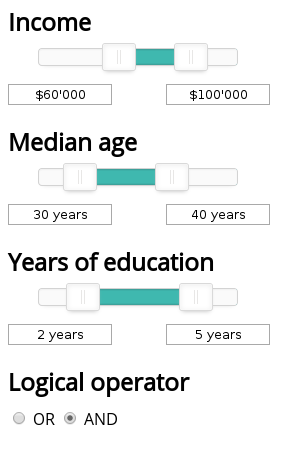
\includegraphics[width=0.35\textwidth]{img/household.png}
  \caption{Panel for filtering housholds.}
  \label{fig:household}
\end{figure}
For filtering the potential households, the GIS operator will be provided with three value sliders representing thresholds for income, age and education. In addition to this, the operator will be able to select how these values are combined. More specifically, combining the values with the logical OR-operator would display parcels which fall in to either of the specified categories, and the logical AND-operator would only display households which are within all three thresholds. Figure~\ref{fig:household} shows a potential interface of filter parameters of households.

For businesses, the same techniques as for parcels would be used, except for the change of profitability attributes. The software would supply sliders for number of employees and total revenue, and provide the same AND/OR switch.

If one have access to the Esri tapestry data, this step could also contain a mechanism that let the operator pick which segment types to show and which to hide.

The result of this step is a reduced set of parcels or businesses shown in the map.

\subsection{Competitors}
\label{sub:Competitors}
As previously discussed, areas where competitors already are providing broadband are associated with high risk and low profitability. To address this issue, the GIS is provided with two more thresholds: Number of ISPs in the area and average connection speed, both of which attributes are from the National Broadband Map. Areas with fewer competitors might be easier to enter, and households and businesses with low internet speeds are more likely to upgrade to a better ISP.

\subsection{Proximity to existing network infrastructure}
\label{sub:Proximity to existing network infrastructure}
\begin{figure}
  \centering
  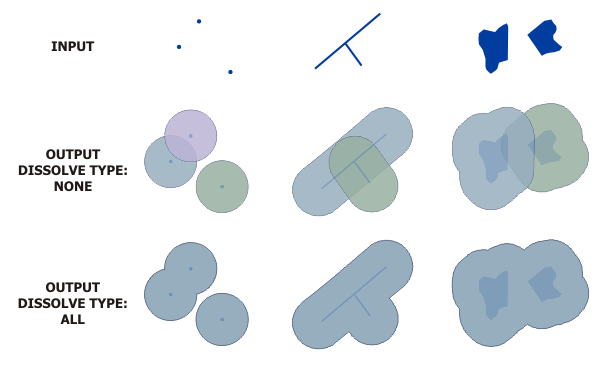
\includegraphics[width=0.45\textwidth]{img/buffer.png}
  \caption{The buffer operation. Create buffer polygons around the input features. Courtesy of \cite{noauthor_undated-ar}.}
  \label{fig:buffer}
\end{figure}
The GIS operator now displays households and businesses with high potential for areas with limited competition from other ISPs. In order to find the customers close to existing network infrastructure, a GIS technique called buffer will be used. This technique, as Figure \ref{fig:buffer} shows, is meant create buffer polygon of a certain distance around the existing network, where the distance is specified with yet another slider in the GIS operator's control. The buffer polygons will not be visible, but rather used to filter households and businesses so the map only displays the ones that intersect the buffer, that is the potential customers within the given distance. 
\subsection{Customer clustering}
\label{sub:Customer clustering}
\begin{figure}
  \centering
  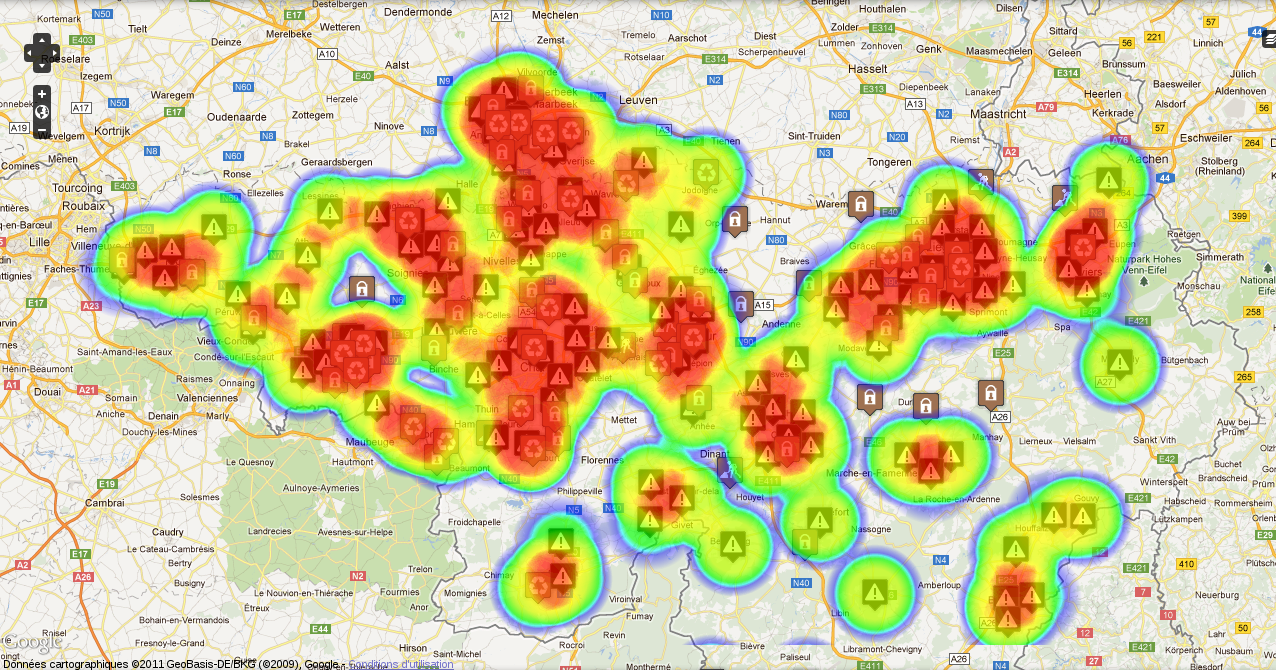
\includegraphics[width=0.45\textwidth]{img/heatmap.png}
  \caption{Heatmap: Source (to be fixed): https://www.drupal.org/files/snapshot15.png}
  \label{fig:heatmap}
\end{figure}
\begin{figure}
  \centering
  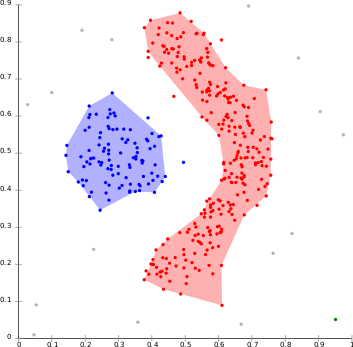
\includegraphics[width=0.40\textwidth]{img/dbscan.png}
  \caption{Density-based clustering. Courtesy of \cite{Wikipedia_contributors2014-qv}.}
  \label{fig:dbscan}
\end{figure}
With all the filters in place, we must now pay attention to the clustering of the remaining customers. This can be done already by simply inspecting the map, looking for several households or businesses in the same area. Depending on how large area is analysed, this process can be tedious and necessarily not accurate. This project therefore proposes two related techniques to aid the operator to find customer clusters.

The first technique is to visualize the clusters as a heat map, like shown in Figure \ref{fig:heatmap}. In this technique, each point, or customer, will contribute with color gradient to the heat map. The more points in the proximity of each other, the stronger the color, which makes it easy to find clusters in the map.

The second one is to use mathematical cluster analysis \cite{Wikipedia_contributors2014-qv}, the task of grouping a set of objects in such way that objects in the same group, or cluster, are more similar than those of other clusters. A way to to it would be to use a density-based clustering algorithm, more specifically algorithms that define clusters where points have higher density are grouped together, like in Figure \ref{fig:dbscan}. In a map, this could be visualized by coloring each cluster differently and adding labels of how many items in the cluster to bring the operator's attention to the area with the most customers.

None of the visualization techniques need any input parameters, but the operator must be able to turn them on or off.

\subsection{Data analysis}
\label{sub:Data analysis}
The GIS operator is now equipped with several filters to adjust. Even though the filters were presented like they were steps, they're not. The operator can adjust any filters in any order he or she would like. Finding the best areas would be a process of trial and error, where several thresholds will have to be continiously adjusted.

\subsection{Profitability score: An alternative method}
\label{sub:Profitability score: An alternate method}
The problem by the current method is that it might completely disregard highly potential customers with only one attribute outside the threshold. An example of this is a cluster of 100 households with only one, slow internet provider, which is located outside the distance bounds of the existing network infrastructure. Even though the cluster is outside the initial bounds, it would possibly still be worthwile to dig the extra distance because the customers scores high on other attributes.

A technique to avoid this situation, would be to pre-calculate a profability score for each business and household. The score would be a formula consisting of all the attributes, and is thought to be normalized, so the most profitable customer has a score of 100\%. The formula will use a linear combination of the input variables, so even though one attribute value is low, it can still get a good score if the rest are good. The GIS operator would then be able to filter this score instead of the individual attributes, effectively avoiding the problem from the previous paragraph. Additionally, this method would be more suitable for pure computer analysis, because the computer can easily pick out the customers with the highest score.

The major downside of this method is the calculation of the profitability score. The formula would need to be carefully crafted so that each attribute weighs in differently. Finding these weights, however, is non-trivial. There's no way one can know in advance how much each attribute should contribute to the final score, so these weights would have to be adjustable. This could be done by providing the GIS operator with sliders, but it is however needless to say that these are far less intuitive than the threshold sliders in the original solution.


\section{Risk assessment and potential pitfalls}
\label{sec:Risk assesment and potential pitfalls}
There are several risks connected to this project. The first of them regards the accuracy of the aquired data. As we know, much of the data for ranking customer profitability comes from coarse-grained data sources, that is data based on census tracts, counties or other divisions to preserve anonymity. This might not be good enough for this appliacition. For instance, there could be severe differences between income and median age in households within a census tract, differences it would be beneficial to pick up, but we're unable to.

A second aspect is the temporal accuracy of the data sources. Extending the customer portolio in newly built neighbourhoods or business areas might be particulary interesting, but relevant data about these locations might not be accurate or even available. Additionally, if the National Broadband Map does not pick up changes in a timely manner, you might end up basing your desicions on outdated data about potential competitors which could have severe consequences.

Lastly, there's a chance we're looking at the wrong attributes. The reasoning in Section \ref{sec:Potential and profitability} is meant to provide guidelines for which attributes are worth paying extra attention to, and should not be considered as an absoulute measure for profitability and potential. It is however worth noting that the system is easily adjustable for new attributes which the ISP finds more useful.

\section{Conclusion}
\label{sec:Conclusion}
\textit{yet to be completed, might be skipped}

\printbibliography

\end{document}
